\newpage
\subsection{Propuesta de solución}

\vspace*{\fill}
\noindent
\begin{figure}[htb]
    \centering
    \makebox[\textwidth]{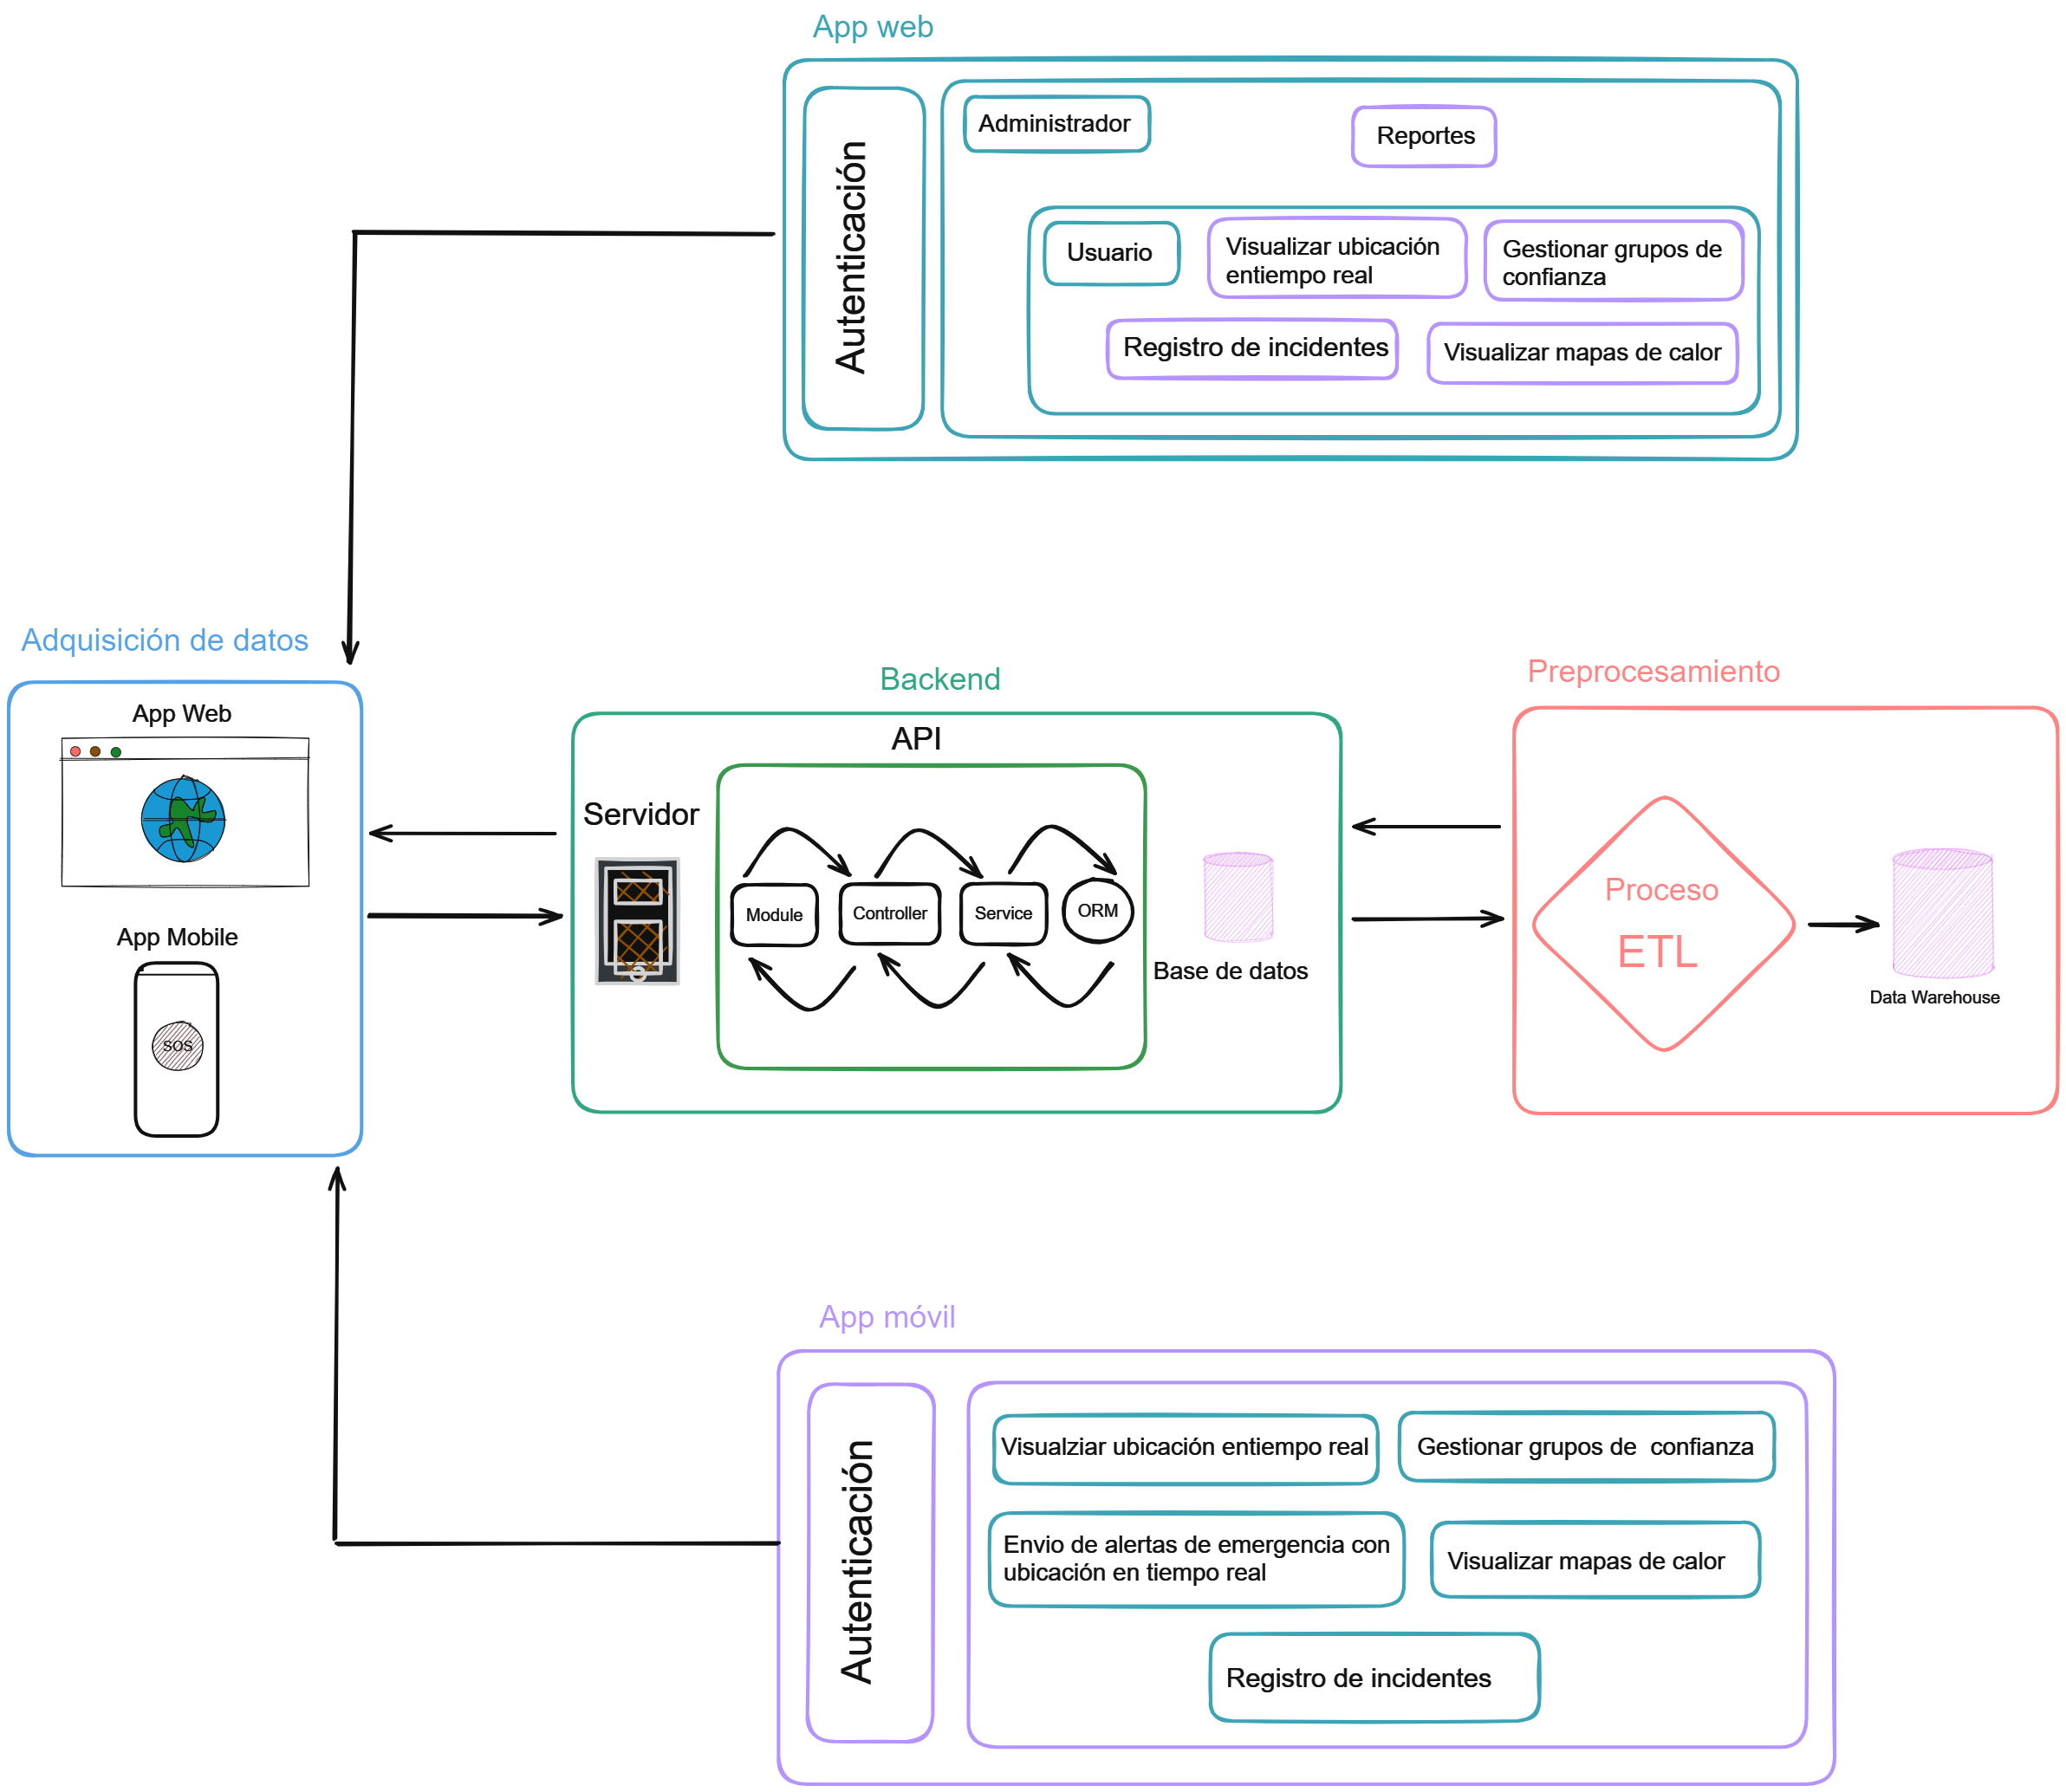
\includegraphics[width=18cm, height=16cm]{./resources/images/esquema.png}}%
    \caption{Esquema del sistema}
    \label{fig:esquema}
\end{figure}


Se propone el desarrollo de una aplicación móvil dedicada a recopilar datos georreferenciados
sobre delitos, mediante alertas de emergencia que incluyan la ubicación en tiempo real. Además,
se integrarán formularios para obtener información detallada de incidentes pasados. Esta aplicación
también administrará grupos de confianza y permitirá el monitoreo en tiempo real de la ubicación
de familiares en situaciones de riesgo, así como la visualización de mapas que identifiquen
zonas conflictivas. Adicionalmente, se planea el desarrollo de una aplicación web complementaria
que posibilite la visualización en tiempo real de familiares en peligro, junto con la capacidad
de registrar incidentes y visualizar mapas de calor que muestren áreas de alta incidencia delictiva.
Esta aplicación web contará con un sistema de roles, donde el administrador tendrá acceso a reportes
detallados sobre los siniestros reportados. Ambas aplicaciones estarán interconectadas con un
servidor que proporcionará una API REST, la cual estará vinculada a una base de datos relacional.
La información recolectada en esta base de datos pasará por un proceso de Extracción, Transformación
y Carga de datos (ETL)  para generar un almacén de datos (data warehouse) y posteriormente un cubo
OLAP. Este cubo OLAP será la fuente primaria de información para la generación de reportes detallados
sobre la incidencia delictiva.